
    

 \section{Model Implementations}   
To make optimization of models tractable it was important to do ongoing feasibility testing. For example its important to evaluate the the utility of established model implementations, as using these models to optimize may not in fact be feasible.\\ 
\\
Despite an abundance of choices in the simple modelling
ecosystem, many off the shelf implementations were not useful, or significant intervention was required to make some established implementations workable inside an optimization framework. \\
\\
In two classes of model a feasible choice of implementation did not exist and it was easier to re-implement those models. The two models I re-implemented were
the Adaptive Exponential Integrate and fire Model, and also the IZHI
model.  In the work below, I profile existing model implementations, and
justify the reasons for re-implementing.\\
\\
This is in contrast to the brian2/neuraldynamics AdExp model, which took
between 2 or 3 times longer to find a rheobase current injection value. However the slowness is not caused by the simulation backend (brian2 which is relatively fast and efficient). The slow down is caused by the way the model is defined. Specifically the
model is defined in a middle code layer neurodynamics\cite{gerstner2014neuronal}.\\
\\
It is very likely, that the model implementation is correct, since Gerstner is an author of one of the original adaptive exponential publications, and the neural dynamics book that the brian2 code is strongly affiliated with. Since Integrate and Fire models don't formally include spikes when an implementation does include spikes, it is an optional add on.\\
\\
The AdExp neurodynamics models default implementation causes spikes with peaks below $0mV$, since the AdExp model like all integrate and fire models do not explicitly include spikes\\
\\
This is not technically wrong, but it violates
assumptions in the \emph{NeuronUnit} feature extraction protocol. The default spiking behavior, looks odd, and it is simply this poor model definition that is causing a slower optimizer performance. The optimizer takes an unusual waveform shape, and searches for longer in distant
parameter regions to find a good fit.\\
\\
Over  the course of evaluating the brian neural dynamics model \cite{gerstner2014neuronal}. I experienced some phenomena that only occurred in the context of genetic algorithm optimization. The reason why optimization provides a different evaluation context is because, in optimization simulation objects are required to be created and destroyed rapidly and on mass. Brian2 is designed to be an efficient network simulator, the case of being designed for network simulation, may assume you will want to create a lot of neural models that persist efficiently together in memory (this was also a problem with PyNN models). Therefore you might see below, that while only one brian model exists in memory, performance is okay, but when creating and destroying models rapidly and on mass a slow down occurs.\\
\\
Below I have implemented a python integrator for the Adaptive
Exponential Integrate and fire model. This solver lead to faster
evaluations of current injection experiments. The integrator I developed
had a $0mV$ spiked when evaluated at default
parameter values.\\


Brian2 and sciunits sometimes collided in name space, and logging.
%\href{https://github.com/scidash/sciunit/pull/124/files/83907ba68740642178ebb91084f6e382e06a43c4#diff-d68791d2ed5dfaa96a900be6180bd950}

\section{Profiling the JIT enabled Adexp Model}
\begin{verbatim}
    

time taken on block 3.3625197410583496

\end{verbatim}

\begin{figure}    
\begin{center}
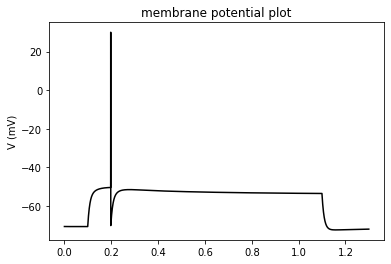
\includegraphics[width=1.1\linewidth]{figures/backend_check_files/backend_check_6_2.png}
\caption{}

\end{center}
\end{figure}

\begin{verbatim}
    251 ms +- 5.02 ms per loop (mean +- std. dev. of 2 runs, 1 loop each)
    240 ms +- 11.1 ms per loop (mean +- std. dev. of 2 runs, 1 loop each)
    223 ms +- 12.5 ms per loop (mean +- std. dev. of 2 runs, 1 loop each)
\end{verbatim}

\begin{verbatim}
    922 ms +- 12.7 ms per loop (mean +- std. dev. of 7 runs, 1 loop each)
\end{verbatim}

\subsection{Compare parallel to serial speeds, and accuracy}

Below is the Brian2/NeuralDynamics AdExp model. In-order to make the spike height greater than $0mV$ it was easier to use computer code to schedule waveform modifications that occur straight after the the brian2 simulation, these scheduled waveform modifictions can be considered part of a peripheral shell of simulation code. In post-processing
the waveform data type is a Neo Wave form object that is artificially
shifted above 0mV using code. The code takes additional time to complete
the algorithm of determining rheobase and displaying results. The time
of this model is deterimant on multiple factors, as discussed elsewhere,
execution time is not uniform across model parameterizations. Models
with multispiking behavior will take longer to solve.

Simulation times for this model vary, dramatically possibly because of
lazy evaluation, the simulation times may vary according to what else
you are running on your computer.

Not all models experience a speed up when executed in parallel, however
this model was faster in the parallel Rheobase determination algorithm.

Some common times are: $3.92,6.75,4.48,5.17$. Mean time was:

\section{Comparison of Times Taken to Find Rheobase}
Custom implementation JIT enabled implementation: $4.0s$. 
Brian2 taken to find Rheobase: $4.40s$ (serial), $3.976s$ (parallel).

The evaluation times between Brian2 and the custom written
integrator are similar. Both have average runs of approximately 4 seconds, however the spike shape derived from the custom implementation look more realistic under initial/default paramaterizations, and the realism of default model paramaterization actually has consequences for model optimization speed.\\

    \begin{center}
    \begin{figure}
    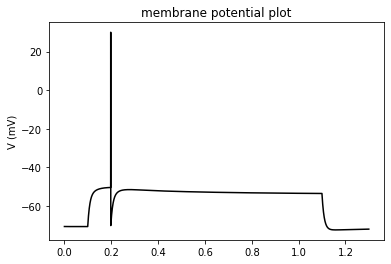
\includegraphics{figures/backend_check_files/backend_check_4_2.png}
    \end{figure}
    \end{center}

\begin{center}
\begin{figure}

    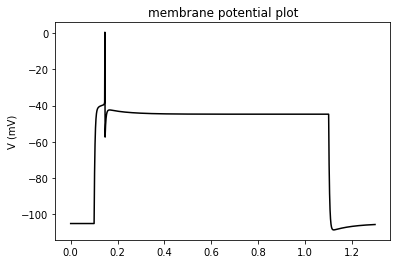
\includegraphics{figures/backend_check_files/backend_check_12_10.png}
\end{figure}

\end{center}
    
\begin{verbatim}
    272 ms +- 66.5 $/mu$s per loop (mean +- std. dev. of 2 runs, 1 loop each)
    303 ms +- 10.9 ms per loop (mean +- std. dev. of 2 runs, 1 loop each)
    342 ms +- 11 ms per loop (mean +- std. dev. of 2 runs, 1 loop each)
\end{verbatim}

The next model to be evaluated is the NEURON Izhi model. The NEURON Izhi model has various draw backs. 1. It depends on an external file which must be recompiled each time this project is recreated. 2. The build environment of NEURON is non-trivial, and only a super dedicated NEURON modeller would install it on their system. Any performance advantage of using NEURON investment does not exceed the installation cost of installing the program. 3. The model implementation code is less generalizable than than the published Izhi model itself. Where the standard NEURON-NeuroML code only covers the Regular-Spiking model * This is likely due to a name space conflict between Capacitance. Neuron has a `capacitive' mechanism inside modelled Neurons, this particular model has section capacitance as well as an introduced capacitive term inside a C-compiled mechanism. Both contribute to a the membrane
potential calculation. * The NEURON Izhi model took $78$ seconds to find the rheobase current injection value.
    
\begin{center}
    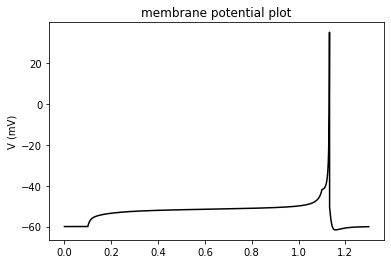
\includegraphics{figures/backend_check_files/backend_check_14_2.png}
\end{center}


\begin{verbatim}
51.79367065 * $pA$
\end{verbatim}
        


\section{Parallel Rheobase}


\begin{figure}    
  \begin{center}
  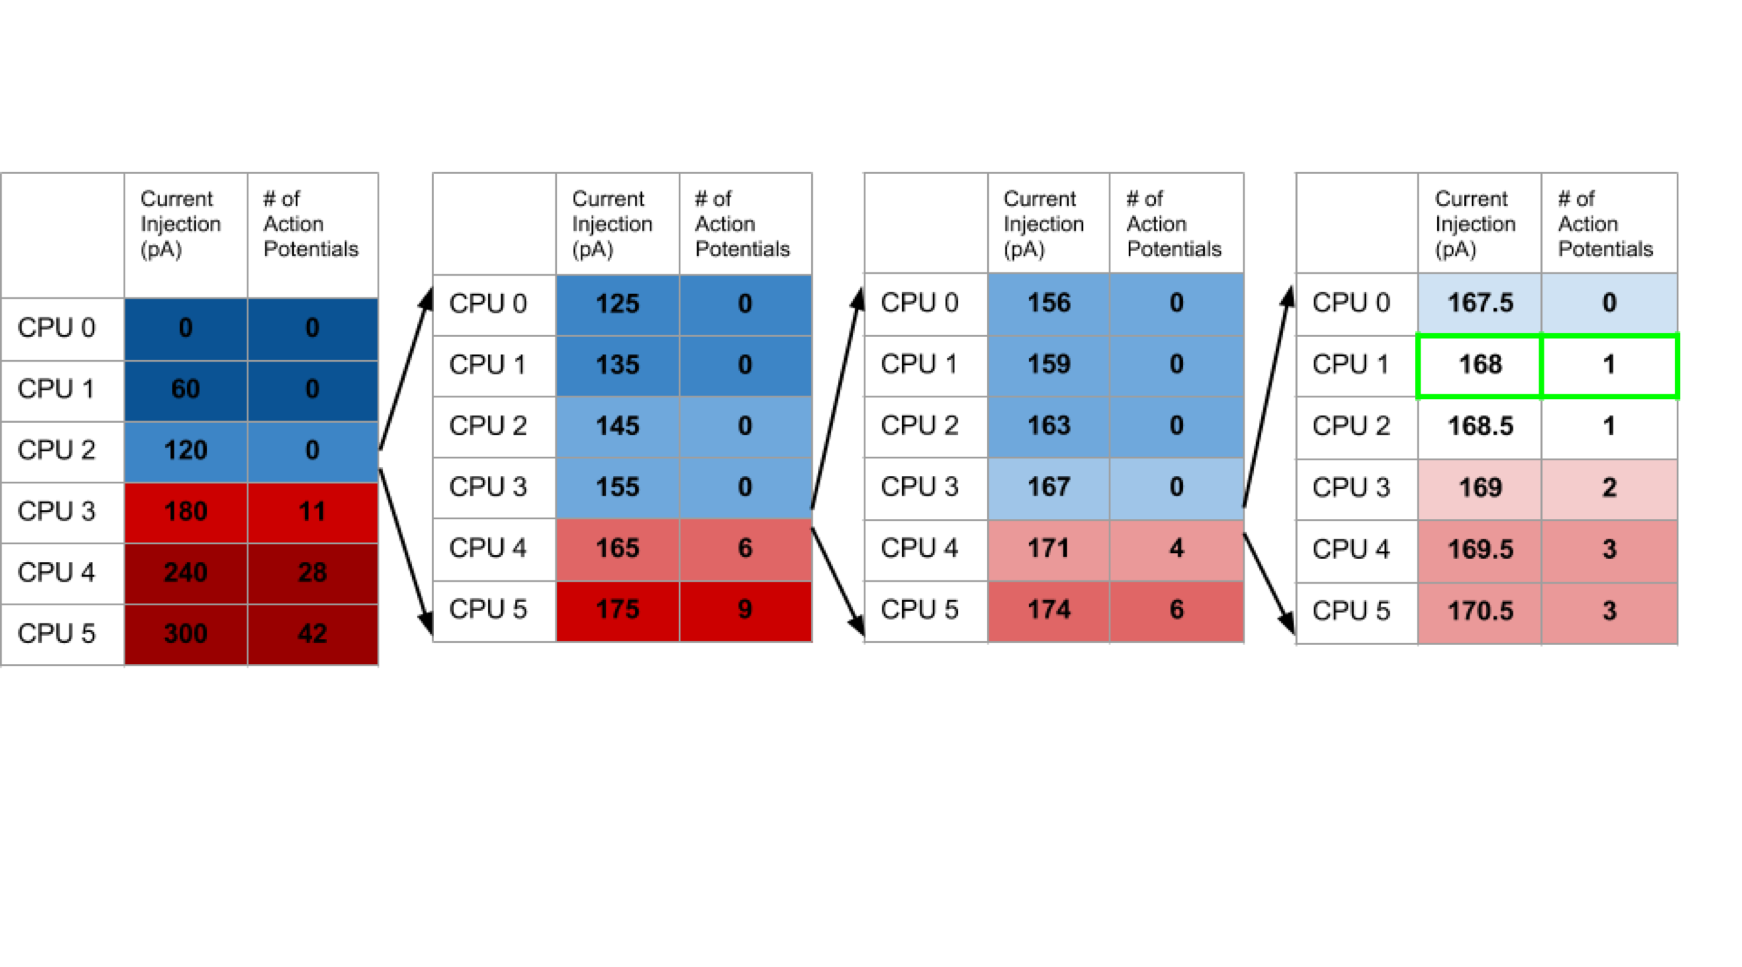
\includegraphics[width=0.7\linewidth]{figures/rheobase_algorithm.png}
    \caption{We developed a generic algorithm which took models, and found the minimal current injection value that would cause only one spike. The normal structure of this algorithm is a binary search, however we modified the algorithm so it would map onto multiple processors at once. This lead to significant speed ups for multicompartment NEURON models}

  \end{center}
\end{figure} 

Algorithm was able to speed up this slow NEURON unit code. 73/19
represents a substantial speed up. of about 3.8. This is consistent with
previous work

\begin{verbatim}
\{'value': array(51.79317142) * pA\}
\end{verbatim}
        
    The forward Euler python IZhi model is very fast. The forward euler
implementation utilized Numba JIT. Rheobase is found in under a second,
and in many cases close 0.5 seconds. This represents a very dramatic
speed up.

Unlike the NEURON NeuroML implementation of the izhikitich equation,
this implementation is just as generalizable as the original MATLAB
implementation of the izhikitich model.


\begin{verbatim}
  time taken on
  block 0.6859951019287109 \textbackslash{}n3.3 ms +- 9.79 $\mu$s per loop (mean +- std. dev. of 2
  runs, 100 loops each)\textbackslash{}n3.32 ms +- 30.9 us per loop (mean +- std. dev. of 2 runs,
  100 loops each)\textbackslash{}n3.19 ms +- 10.9 us per loop (mean +- std. dev. of 2 runs, 100

\end{verbatim}
        
\section{Python/LEMS and NEURON versions of single compartment Conducance Model.}

Conductance based models took approximately the same amount of
time to evaluate the Rheobase search algorithm as the python
implementation.

%This problem in the default parameterization of the python model was later located in the scale or units of capacitance, if default capacitance parameterization is multiplied by 100.0 the problem goes away.

\begin{verbatim}
time taken on block $ 12.6s $
\end{verbatim}

\begin{center}
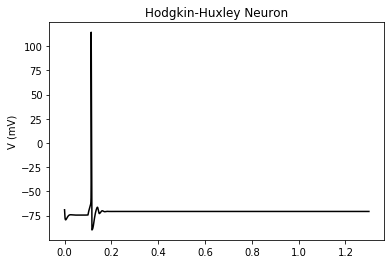
\includegraphics{backend_check_files/backend_check_22_2.png}
\end{center}

\begin{verbatim}
1.40762329 * pA
\end{verbatim}


\subsection{NEURON versions of single compartment Conducance
model.}

Conductance based chanels models took approximately the same amount of time to evaluate the Rheobase search algorithm as the python
implementation.

The NEURON implementation was slightly faster, and the default
parameterization of the model lacked ``ringing'', or below threshold
oscillations that the Python ODE version had under default conditions.

This problem in the default parameterization of the python model was
later located in the scale or units of capacitance, if default
capacitance parameterization is multiplied by 100.0 the problem goes
away.

    \begin{verbatim}
time taken on block 8.573923826217651
    \end{verbatim}


    
    \begin{center}
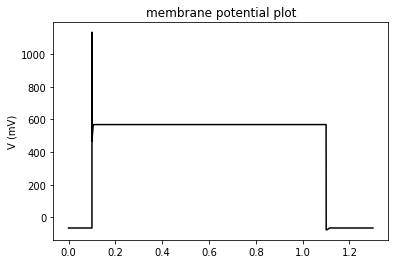
\includegraphics{figures/backend_check_files/backend_check_26_2.png}
    \end{center}
\begin{verbatim}
112.5 pA
'value': array(1.40645904) * pA
\end{verbatim}


\begin{verbatim}
\{'El\_reference': -0.07016548013687134, 'C': 3.990452661875942e-10,
'init\_threshold': 0.02964956889477108, 'th\_inf': 0.02964956889477108,
'spike\_cut\_length': 109.5, 'init\_voltage': -35.0, 'R\_input': 910258965.9792937\}
0.62137434895311 mV 2.7368671294272984 mV
0.0 mV -0.065 mV
0.31069759691841936 mV 1.33594806210705 mV
0.15535922090107404 mV 0.6354885284469255 mV
0.07769003289240137 mV 0.28525876161686337 mV
0.07769003289240137 mV 0.28525876161686337 mV
time taken on block 0.23476457595825195
\end{verbatim}

    

    
    \begin{center}
    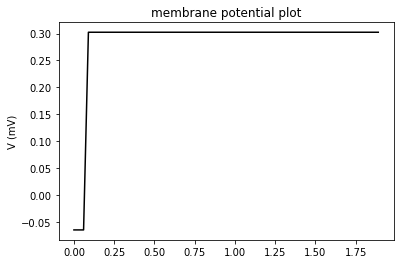
\includegraphics{backend_check_files/backend_check_28_3.png}
    \end{center}
    \begin{verbatim}
    112.5 pA
    \end{verbatim}

    $0.0 mV$ $-0.065 mV$

    \begin{verbatim}
    0.12659285497193595 mV 0.5057737999913468 mV
    0.3797368751483505 mV 1.6472634104004382 mV
    0.2531648650601433 mV 1.0765186051958928 mV
    \{'value': array(183.33333333) * pA\}
    \end{verbatim}

\begin{verbatim}
array(112.5) * pA
\end{verbatim}


\begin{verbatim}
    0.017240506310425608 mV -0.08583939747094235 mV
    0.017240506310425608 mV -0.08583939747094235 mV
\end{verbatim}

    \begin{center}
    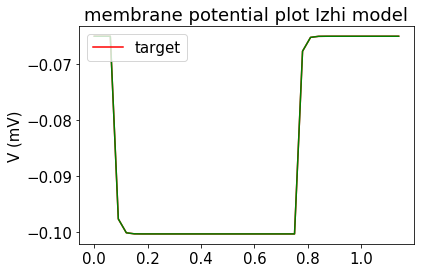
\includegraphics{figures/backend_check_files/backend_check_32_2.png}
    \end{center}
